\documentclass[dvipdfmx]{ujarticle}
\usepackage{eee}

\begin{document}
\title{平成30年 電磁気学II}
\date{}
\author{大山主朗}

\maketitle

\section*{平成30年 電磁気学II 第1回小テスト}
\section{以下の(a)及び(c)に示す物理定数は電磁気学を修めた者であれば常識的に覚えていなければならない数値である.それぞれの値を示せ.}
\begin{enumerate}[(a)]
	\item 真空の誘電率$\varepsilon_{0}:8.854 \times 10^{-12}\,\rm{F/m}$
	\item 真空の透磁率$\mu_{0}:1.257 \times 10^{-6}\,\rm{H/m}$
	\item 電子の電荷$e:-1.602 \times 10^{-19}\,\rm{C}$
\end{enumerate}

\section{一辺の長さ$a$の正方形がある.点Aに$-2q[\rm{C}]$,点Bに$+1q[\rm{C}]$,点Cに$−4q[\rm{C}]$,点Dに$+3q[\rm{C}]$,が点Oに$-q[\rm{C}]$の点電荷が存在するとき,点Oにある電荷にはたらく力$F$の大きさを求めよ.ただし,$q>0$とする.}
\begin{align*}
		\boldsymbol{F}_{A}&=\frac{1}{4\pi \varepsilon_{0}}\frac{-2q(-q)}{\left(\left(-\frac{a}{2}\right)^{2}+\left(\frac{a}{2}\right)^{2}\right)^{3/2}} \left\{-\frac{a}{2}\boldsymbol{i}+\frac{a}{2}\boldsymbol{j}\right\}\,[\rm{N}]\\
		\boldsymbol{F}_{B}&=\frac{1}{4\pi \varepsilon_{0}}\frac{q(-q)}{\left(\left(-\frac{a}{2}\right)^{2}+\left(-\frac{a}{2}\right)^{2}\right)^{3/2}} \left\{-\frac{a}{2}\boldsymbol{i}-\frac{a}{2}\boldsymbol{j}\right\}\,[\rm{N}]\\
		\boldsymbol{F}_{C}&=\frac{1}{4\pi \varepsilon_{0}}\frac{-4q(-q)}{\left(\left(\frac{a}{2}\right)^{2}+\left(-\frac{a}{2}\right)^{2}\right)^{3/2}} \left\{\frac{a}{2}\boldsymbol{i}-\frac{a}{2}\boldsymbol{j}\right\}\,[\rm{N}]\\
		\boldsymbol{F}_{D}&=\frac{1}{4\pi \varepsilon_{0}}\frac{3q(-q)}{\left(\left(\frac{a}{2}\right)^{2}+\left(\frac{a}{2}\right)^{2}\right)^{3/2}} \left\{\frac{a}{2}\boldsymbol{i}+\frac{a}{2}\boldsymbol{j}\right\}\,[\rm{N}]\\
		\boldsymbol{F}&=\boldsymbol{F}_{A}+\boldsymbol{F}_{B}+\boldsymbol{F}_{C}+\boldsymbol{F}_{D}\\
		&=\frac{1}{4\pi \varepsilon_{0}}\frac{q^{2}}{\left(\left(\frac{a}{2}\right)^{2}+\left(\frac{a}{2}\right)^{2}\right)^{3/2}}\left\{\left(-a+\frac{a}{2}+2a-\frac{3}{2}a\right)\boldsymbol{i}+\left(a+\frac{a}{2}-2a-\frac{3}{2}a\right)\boldsymbol{j}\right\}\\
		&=\frac{1}{4\pi \varepsilon_{0}}\frac{q^{2}}{\left(\frac{a^{2}}{4}\right)^{3/2}}\left(-2a\boldsymbol{j}\right)\\
		&=\frac{1}{4\pi \varepsilon_{0}}\frac{8q^{2}}{a^{3}}\left(-2a\boldsymbol{j}\right)\\
		&=-\frac{4q^{2}}{\pi \varepsilon_{0}a^{2}}\,\boldsymbol{j}\,[\rm{N}]\\
		|\boldsymbol{F}|&=\frac{4q^{2}}{\pi \varepsilon_{0}a^{2}}\,[\rm{N}]\quad y軸下向き
\end{align*}

\section{一辺の長さ$a$の正方形がある.点Bに$+m[\rm{Wb}]$,点Cに$−3m[\rm{Wb}]$,点D に $+2m [\rm{Wb}]$,点Oに $+m[\rm{Wb}]$の点磁荷が存在するとき,点Aにできる磁界$H$の大きさを求めよ.ただし,$m >0$とする.}
\begin{align*}
		\boldsymbol{H}_{O}&=\frac{1}{4\pi \mu_{0}}\frac{m}{\left(\left(-\frac{a}{2}\right)^{2}+\left(\frac{a}{2}\right)^{2}\right)^{3/2}} \left\{-\frac{a}{2}\boldsymbol{i}+\frac{a}{2}\boldsymbol{j}\right\}\\
		&=\frac{1}{4\pi \mu_{0}}\frac{m}{\left(\frac{a^{2}}{2}\right)^{3/2}} \left\{-\frac{a}{2}\boldsymbol{i}+\frac{a}{2}\boldsymbol{j}\right\}\\
		&=\frac{m\sqrt{2}}{4\pi \mu_{0} a^{2}}\left\{-\boldsymbol{i}+\boldsymbol{j}\right\}\,[\rm{A/m}]\\
		\boldsymbol{H}_{B}&=\frac{1}{4\pi \mu_{0}}\frac{m}{\left(a^{2} \right)^{3/2}}a\boldsymbol{j}\\
		&=\frac{m}{4\pi \mu_{0}a^{2}}\boldsymbol{j}\,[\rm{A/m}]\\
		\boldsymbol{H}_{C}&=\frac{1}{4\pi \mu_{0}}\frac{-3m}{\left((-a)^{2}+a^{2} \right)^{3/2}}\left\{ -a \boldsymbol{i}+a\boldsymbol{j}\right\}\\
		&=\frac{1}{4\pi \mu_{0}}\frac{-3m}{2\sqrt{2}a^{3}}\left\{ -a \boldsymbol{i}+a\boldsymbol{j}\right\}\\
		&=\frac{-3m}{8\sqrt{2} \pi \mu_{0} a^{2}}\left( -\boldsymbol{i}+\boldsymbol{j}\right)\,[\rm{A/m}]\\
		\boldsymbol{H}_{D}&=\frac{1}{4\pi \mu_{0}}\frac{2m}{\left((-a)^{2} \right)^{3/2}}\left(-a\boldsymbol{i}\right)\\
		&=-\frac{m}{2\pi \mu_{0}a^{2}}\boldsymbol{i}\,[\rm{A/m}]\\
		\boldsymbol{H}&=\boldsymbol{H}_{O}+\boldsymbol{H}_{B}+\boldsymbol{H}_{C}+\boldsymbol{H}_{D}\\
		&=\frac{m}{2\pi \mu_{0}a^{2}}\left\{\left(-\frac{\sqrt{2}}{2}+\frac{3}{4\sqrt{2}}-1\right)\boldsymbol{i}+\left(\frac{\sqrt{2}}{2}+\frac{1}{2}-\frac{3}{4\sqrt{2}}\right)\boldsymbol{j} \right\}\\
		&=\frac{m}{2\pi \mu_{0}a^{2}}\left\{\left(\frac{-8-\sqrt{2}}{8}\right)\boldsymbol{i}+\left(\frac{4+\sqrt{2}}{8}\right)\boldsymbol{j} \right\}\\
		&=\frac{m}{16\pi \mu_{0}a^{2}}\left\{-\left(8+\sqrt{2}\right)\boldsymbol{i}+\left(4+\sqrt{2}\right)\boldsymbol{j} \right\}\\
		|\boldsymbol{H}|&=\frac{m}{16\pi \mu_{0}a^{2}}\sqrt{(8+\sqrt{2})^{2}+(4+\sqrt{2})^{2}}\\
		&=\frac{m}{16\pi \mu_{0}a^{2}}\sqrt{84+24\sqrt{2}}\\
		&=\frac{m}{8\pi \mu_{0}a^{2}}\sqrt{21+6\sqrt{2}}\,[\rm{A/m}]\quad 左斜め上向き
\end{align*}

\section{以下の(a)から(c)に示すような電荷分布が存在するとき,それぞれの電荷分布が周囲につくる電界$E$をガウスの法則を用いて求めよ.}
\begin{enumerate}[(a)]
	\item $q\,[\rm{C}]$の点電荷
	\begin{align*}
		\oint_{S} E_{n} dS&=\frac{1}{\varepsilon_{0}} \sum_{i} Q_{i}\\
		E_{n}&=\frac{q}{4\pi \varepsilon_{0} r^{2}}\,[\rm{V/m}]
	\end{align*}
	\item 線電荷密度$\lambda\,[\rm{C/m}]$で分布する無限長直線電荷
	\begin{align*}
		\oint_{S} E_{n} dS&=\frac{1}{\varepsilon_{0}} \sum_{i} Q_{i}\\
		E_{n}&=\frac{\lambda l}{2\pi \varepsilon_{0}r l}\\
		&=\frac{\lambda}{2\pi \varepsilon_{0}r}\,[\rm{V/m}]
	\end{align*}
	\item 面電荷密度$\sigma\,[\rm{C/m^{2}}]$の無限長面電荷
	\begin{align*}
		\oint_{S} E_{n} dS&=\frac{1}{\varepsilon_{0}} \sum_{i} Q_{i}\\
		E_{n}&=\frac{\sigma S}{\varepsilon_{0}S}\\
		&=\frac{\sigma}{\varepsilon_{0}}\,[\rm{V/m}]
	\end{align*}
\end{enumerate}

\section{導体板の面積$S$,導体板の平行平板キャパシタの内部が比誘電率$\varepsilon_{r}$の誘電体で満たされているとき,この平行平板キャパシタの静電容量$C$が$C=\varepsilon_{0}\varepsilon_{r}\frac{S}{d}$で求められる理由を説明せよ.}
電極に$\pm Q$の電荷を与える.次に,電極間に発生する電界$E$を求め,電極間の電圧$V$を求める.
それらを,$C=\frac{Q}{V}$に代入すことにより,与式が導出される.
\begin{align*}
	C&=\frac{Q}{V}\\
	&=\frac{Q}{Ed}\\
	&=\frac{Q}{\frac{Qd}{\varepsilon_{0}\varepsilon_{r}S}}\\
	&=\varepsilon_{0}\varepsilon_{r}\frac{S}{d}\,[\rm{F}]
\end{align*}

\section{真空中に単磁荷$m$が存在する.ただし$m<0$とする.このとき以下の問いに答えよ.}
\begin{enumerate}[(a)]
	\item 点磁荷$m$が,距離$r$の位置に作る磁界$H$を求めよ.
	\begin{align*}
		H&=\frac{m}{4 \pi \mu_{0} r^{2}}\,[\rm{A/m}]
	\end{align*}
	\item 点磁荷$m$が作る磁界の様子を磁力線を用いて図示せよ.
	\begin{figure}[h]
	\centering
	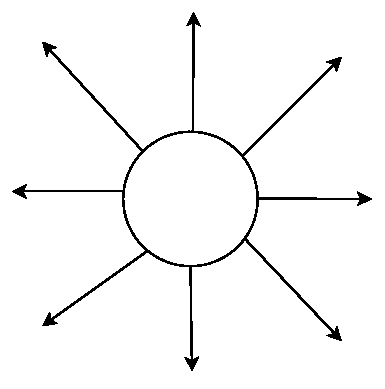
\includegraphics[scale=1]{./efig.pdf}
	\end{figure}
	\item 点磁荷$m$から距離$r$の位置における磁束密度$B$を求めよ.
	\begin{align*}
		B&=\mu_{0} H=\frac{m}{4 \pi r^{2}}\,[\rm{T}]
	\end{align*}
	\item 点磁荷$m$から距離$r$の位置を通過する磁束$\Phi$を磁束密度$B$より求めよ.
	\begin{align*}
		\Phi&=BS=m\,[\rm{Wb/m}]
	\end{align*}
\end{enumerate}

\section{$xy$直交座標系において,同量異符号の点磁荷$\pm m$が距離$l$に固定された磁気双極子が存在する.このとき以下の問いに答えよ.ただし,$x$ 方向の基準ベクトルを$\boldsymbol{i}$,$y$方向の基準ベクトルを$\boldsymbol{j}$とする}
\begin{enumerate}[(a)]
	\item 点Aに存在する磁荷$-m$が点P$(x_0,y_0)$に作る磁界$\boldsymbol{H}_{1}$を求めよ.
	\begin{align*}
		\boldsymbol{H}_{1}&=\frac{1}{4\pi \mu_{0}}\frac{-m}{\left(\left(x_{0}+\frac{l}{2}\right)^{2}+y_{0}^{2}\right)^{3/2}} \left\{ \left(x_{0}+\frac{l}{2}\right)\boldsymbol{i}+y_{0}\boldsymbol{j}\right\}\,[\rm{A/m}]
	\end{align*}
	\item 点Bに存在する磁荷$+m$が点P$(x_0,y_0)$に作る磁界$\boldsymbol{H}_{2}$を求めよ.
	\begin{align*}
		\boldsymbol{H}_{2}&=\frac{1}{4\pi \mu_{0}}\frac{m}{\left(\left(x_{0}-\frac{l}{2}\right)^{2}+y_{0}^{2}\right)^{3/2}} \left\{ \left(x_{0}-\frac{l}{2}\right)\boldsymbol{i}+y_{0}\boldsymbol{j}\right\}\,[\rm{A/m}]
	\end{align*}
	\item 点Pでの磁界$\boldsymbol{H}$を求めよ.
	\begin{align*}
		\boldsymbol{H}&=\boldsymbol{H}_{1}+\boldsymbol{H}_{2}\\
		&=\frac{m}{4\pi \mu_{0}}\left[\frac{-1}{\left(\left(x_{0}+\frac{l}{2}\right)^{2}+y_{0}^{2}\right)^{3/2}} \left\{ \left(x_{0}+\frac{l}{2}\right)\boldsymbol{i}+y_{0}\boldsymbol{j}\right\}+\frac{1}{\left(\left(x_{0}-\frac{l}{2}\right)^{2}+y_{0}^{2}\right)^{3/2}} \left\{ \left(x_{0}-\frac{l}{2}\right)\boldsymbol{i}+y_{0}\boldsymbol{j}\right\}\right]\,[\rm{A/m}]
	\end{align*}
	\item 磁気双極子モーメント$\boldsymbol{M}$を求めよ.
	\begin{align*}
		\boldsymbol{M}&=m\boldsymbol{l}\\
		&=ml\boldsymbol{i}\,[\rm{Wb\cdot m}]
	\end{align*}
	\item 点Pが原点Oより十分遠方にあると仮定すると,$\sqrt{(x_{0}-l/2)^{2}+y_{0}^{2}}\simeq \sqrt{x_{0}^{2}+y_{0}^{2}}$及び$\sqrt{(x_{0}+l/2)^{2}+y_{0}^{2}} \simeq \sqrt{x_{0}^{2}+y_{0}^{2}}$と近似できる.このことを用いて(c)にて得た磁界$\boldsymbol{H}$を簡略化せよ.
	\begin{align*}
		\boldsymbol{H}&\simeq -\frac{1}{4\pi \mu_{0}}\frac{ml}{\left(x_{0}^{2}+y_{0}^{2}\right)^{3/2}} \boldsymbol{i}\,[\rm{A/m}]\\
		&\left(\simeq -\frac{\boldsymbol{M}}{4\pi \mu_{0}r^{3}}\,[\rm{A/m}]\right)
	\end{align*}
	\item $y$方向に一様な磁界$\boldsymbol{H}_{0}$が存在するとき,磁気双極子にはたらくトルク$T$を求めよ.
	\begin{align*}
		\boldsymbol{T}&=\boldsymbol{M}H_{0}\sin \theta \\
		&=ml\boldsymbol{i}\sin \frac{\pi}{2}\\
		&=ml\boldsymbol{i}\\
		|\boldsymbol{T}|&=ml\,[\rm{Wb\cdot m}],x軸右方向
	\end{align*}
\end{enumerate}

\section{強磁性体,常磁性体,反磁性体の3つの磁性体の性質を,比透磁率と磁化率を用いて説明せよ.}
強磁性体は磁化率が0よりかなり大きく,透磁率が1よりかなり大きい磁性体を指す.そのため,磁界と同じ方向に磁化され,その大きさも大きい.

常磁性体は磁化率が0より大きく,透磁率は1未満の磁性体を指す.そのため,磁界と同じ方向に磁化され,その大きさは大きくない.

反磁性体は磁化率が0より小さく,透磁率が1より小さい磁性体を指す.そのため,磁界と逆方向に磁化され,その大きさは小さい.

\clearpage
\setcounter{section}{0}
\section*{平成30年 電磁気学II 第2回小テスト}
\section{以下の(a)及び(c)に示す物理定数は電磁気学を修めた者であれば常識的に覚えていなければならない数値である.それぞれの値を示せ.}
\begin{enumerate}[(a)]
	\item 真空の誘電率$\varepsilon_{0}:8.854 \times 10^{-12}\,\rm{F/m}$
	\item 真空の透磁率$\mu_{0}:1.257 \times 10^{-6}\,\rm{H/m}$
	\item 電子の電荷$e:-1.602 \times 10^{-19}\,\rm{C}$
\end{enumerate}

\section{磁化されていない強磁性体に磁界$H$を外部から印加し,強磁性体内部での磁束密度$B$を観測すると,図3に示すような結果が得られた.このとき,図中の行程1:点$\rm{O}\to$点$\rm{P_{1}}$,行程 2:点$\rm{P_{1}}\to$点$\rm{P_{2}}$,行程3:点$\rm{P_{2}}\to$点$\rm{P_{3}}$,行程4:点$\rm{P_{3}}\to$点P4,行程5:点P4 $\to$点$\rm{P_{5}}$, 行程6:点$\rm{P_{5}}\to$点P6,行程7:点$\rm{P_{6}}\to$点P1の7つの行程に着目して,測定結果を説明せよ.}

\section{$xyz$直角座標空間において,$y$軸上の点P$(0, h, 0)$を中心とし,$y=h$の平面内に半径$a$の円形ループ電流$I$が流れている.このとき,以下の各問いに答えよ.}
\begin{enumerate}[(a)]
	\item 点Pに発生する磁界$\boldsymbol{H}$を求めよ.
	\begin{align*}
		x方向,y方向,z方向の&基底ベクトルをそれぞれ\boldsymbol{i},\boldsymbol{j},\boldsymbol{k}とする\\
	d\boldsymbol{l}\times \boldsymbol{l}&の方向よりd\boldsymbol{H}はy軸左向き\\
	\boldsymbol{H}&=\oint d\boldsymbol{H}\\
	&=\oint \frac{Id\boldsymbol{I}\times \boldsymbol{r}}{4\pi a^{3}}\\
	&=\frac{I}{4\pi a^{3}} \oint \boldsymbol{r} \times d\boldsymbol{I}\\
	|\boldsymbol{H}|&=\frac{I}{4\pi a^{3}} \oint r \sin \frac{\pi}{2}dl\\
	&=\frac{I}{4\pi a^{2}}2\pi a\\
	&=\frac{I}{2a}\,[\rm{A/m}]\\
	\boldsymbol{H}&=\frac{I}{2a}\boldsymbol{j}\,[\rm{A/m}]
	\end{align*}
	\item 点Oに発生する磁界$\boldsymbol{H}$を求めよ.
	\begin{align*}
		x方向,y方向,z方向の&基底ベクトルをそれぞれ\boldsymbol{i},\boldsymbol{j},\boldsymbol{k}とする\\
			z>0に円周上の&微小磁界d\boldsymbol{H}_{1}を\\
	z<0に円周上の&微小磁界d\boldsymbol{H}_{2}を考える.\\
	またそれぞれの&線素ベクトルをd\boldsymbol{l}ととる.\\
	ここで,d\boldsymbol{H}_{1}とd\boldsymbol{H}_{2}の外積より,&2つの磁界は打ち消される方向となっているため,\\
	d\boldsymbol{H}_{1}とd\boldsymbol{H}_{2}を合成した&磁界をd\boldsymbol{H}とする.(\phi:d\boldsymbol{H}_{2}とd\boldsymbol{H}のなす角)\\
	またd\boldsymbol{H}の向きは&y軸左方向である\\
	|d\boldsymbol{H}_{1}|=|d\boldsymbol{H}_{2}|&=\frac{Idl}{4\pi r^{2}}\sin \theta\\
	&=\frac{Idl}{4\pi (a^{2}+h^{2})}\\
	d\boldsymbol{H}&=2d\boldsymbol{H}_{1}\cos \phi\\
	&=2d\boldsymbol{H}_{1}\frac{a}{r}\\
	&=2d\boldsymbol{H}_{1}\frac{a}{\sqrt{a^{2}+h^{2}}}\\
	|d\boldsymbol{H}|&=2|d\boldsymbol{H}_{1}|\frac{a}{\sqrt{a^{2}+h^{2}}}\\
	&=\frac{aIdl}{2\pi (a^{2}+h^{2})^{3/2}}\\
	\boldsymbol{H}&=\oint d\boldsymbol{H}_{1}\\
	|\boldsymbol{H}|&=\frac{1}{2}\oint|d\boldsymbol{H}|\\
	&=\frac{1}{2}\oint \frac{aIdl}{2\pi (a^{2}+h^{2})^{3/2}}\\
	&=\frac{1}{2}\cdot \frac{aI}{2\pi (a^{2}+h^{2})^{3/2}} \cdot 2\pi a\\
	&=\frac{a^{2}I}{2 (a^{2}+h^{2})^{3/2}}\,[\rm{A/m}]\\
	\boldsymbol{H}&=\frac{a^{2}I}{2 (a^{2}+h^{2})^{3/2}}\boldsymbol{j}\,[\rm{A/m}]
	\end{align*}
	\item (b)で得られた解答$\boldsymbol{H}$を用いて$\int_{-\infty}^{\infty}\boldsymbol{H}dh$を計算せよ.
	\begin{align*}
	\int_{-\infty}^{\infty}\boldsymbol{H}dh&=\int_{-\infty}^{\infty} \frac{a^{2}I}{2(a^{2}+h^{2})^{3/2}}\boldsymbol{j} dh\\
	h&=a\tan \theta と置換する.\\
	\frac{dh}{d\theta}&=\frac{a}{\cos ^{2}\theta } \quad \therefore dh=\frac{a}{\cos ^{2}\theta }d\theta \\
	また積分範囲は&-\infty \to \infty から-\frac{\pi}{2} \to \frac{\pi}{2}に変わる.\\
	&=\int_{-\frac{\pi}{2}}^{\frac{\pi}{2}} \frac{a^{2}I}{2a^{3}(1+\tan^{2}\theta)^{3/2}}\boldsymbol{j} \frac{a}{\cos ^{2}\theta }d\theta\\
	&=\frac{I}{2} \boldsymbol{j} \int_{-\frac{\pi}{2}}^{\frac{\pi}{2}} \frac{1}{(1+\tan^{2}\theta)^{3/2}} \frac{1}{\cos ^{2}\theta }d\theta\\
	&=\frac{I}{2} \boldsymbol{j} \int_{-\frac{\pi}{2}}^{\frac{\pi}{2}} \frac{1}{(\frac{1}{\cos^{2} \theta })^{3/2}} \frac{1}{\cos ^{2}\theta }d\theta\\
	&=\frac{I}{2} \boldsymbol{j} \int_{-\frac{\pi}{2}}^{\frac{\pi}{2}} \cos \theta d\theta\\
	&=\frac{I}{2} \boldsymbol{j} \left\{1-(-1)\right\}\\
	&=I\boldsymbol{j}\,[\rm{A/m}]
	\end{align*}
\end{enumerate}

\section{$xyz$直角座標空間において,$y$軸上の点$\rm{A}(0, c_{1}, 0)$から点$\rm{B}(0, c_{2}, 0)$まで$y$軸に沿って直線状に流れる電流$I$がある.このとき,$x$軸上の点$\rm{P}(a, 0, 0)$に発生する磁界$\boldsymbol{H}$を求めよ.また,電流$I$の始点Aと終点Bの座標がそれぞれ$(0, -\infty, 0), (0, \infty, 0)$となった場合の点$\rm{P}$に発生する磁界$\boldsymbol{H}$を求めよ.}
	\begin{align*}
	x方向,y方向,z方向の&基底ベクトルをそれぞれ\boldsymbol{i},\boldsymbol{j},\boldsymbol{k}とする\\
	この時&d\boldsymbol{l}=dy\boldsymbol{i}, \boldsymbol{r}=a\boldsymbol{i}-y\boldsymbol{j}\\
	d\boldsymbol{l}\times \boldsymbol{r}&=
	\begin{vmatrix}
	\boldsymbol{i} & \boldsymbol{j} & \boldsymbol{k}\\
	0 &dy & 0\\
	a & -y &0
	\end{vmatrix}
	=dy
	\begin{vmatrix}
	\boldsymbol{i}  & \boldsymbol{k}\\
	a & 0
	\end{vmatrix}
	=-ady\boldsymbol{k}\\
	\boldsymbol{H}&=\int_{C} d\boldsymbol{H}\\
	&=-\int_{C} \frac{aI\boldsymbol{k}}{4\pi(a^{2}+y^{2})^{3/2}}dy\\
	&=-\int_{c_{1}}^{c_{2}} \frac{aI\boldsymbol{k}}{4\pi(a^{2}+y^{2})^{3/2}}dy\\
	h&=a\tan \theta と置換する.\\
	\frac{dh}{d\theta}&=\frac{a}{\cos ^{2}\theta } \quad \therefore dh=\frac{a}{\cos ^{2}\theta }d\theta \\
	また積分範囲は&c_{1}\to c_{2}から\alpha-\frac{\pi}{2} \to \beta -\frac{\pi}{2}に変更される.\\
	&=-\int_{\alpha-\frac{\pi}{2}}^{\beta -\frac{\pi}{2}} \frac{a^{2}I}{4\pi a^{3}(1+\tan^{2}\theta)^{3/2}}\boldsymbol{j} \frac{a}{\cos ^{2}\theta }d\theta\\
	&=-\frac{I}{4\pi} \boldsymbol{k}\int_{\alpha-\frac{\pi}{2}}^{\beta -\frac{\pi}{2}} \frac{1}{(1+\tan^{2}\theta)^{3/2}} \frac{1}{\cos ^{2}\theta }d\theta\\
	&=-\frac{I}{4\pi a} \boldsymbol{k} \int_{\alpha-\frac{\pi}{2}}^{\beta -\frac{\pi}{2}} \frac{1}{(\frac{1}{\cos^{2} \theta })^{3/2}} \frac{1}{\cos ^{2}\theta }d\theta\\
	&=-\frac{I}{4\pi a} \boldsymbol{k}\int_{\alpha-\frac{\pi}{2}}^{\beta -\frac{\pi}{2}} \cos \theta d \theta \\\
	&=-\frac{I}{4\pi a} \left[\sin \theta  \right]_{\alpha-\frac{\pi}{2}}^{\beta -\frac{\pi}{2}}\boldsymbol{k}\\
	&=-\frac{I}{4\pi a}\left\{\sin \left(\beta -\frac{\pi}{2}\right) -\sin \left(\alpha-\frac{\pi}{2}\right) \right\}\boldsymbol{k}\\
	&=-\frac{I}{4\pi a} \left(-\cos \beta +\cos \alpha \right)\boldsymbol{k}\\
	&=-\frac{I}{4\pi a} \left(\cos \alpha -\cos \beta \right)\boldsymbol{k}\,[\rm{A/m}]\\
	始点Aと終点B&の座標がそれぞれ(0, -\infty, 0), (0, \infty, 0)の場合は\\
	\alpha=0,&\beta =\pi であるので\\
	\boldsymbol{H}&=-\frac{I}{4\pi a}\cdot 2 \boldsymbol{k}\\
	&=-\frac{I}{2\pi a} \boldsymbol{k}\,[\rm{A/m}]
	\end{align*}
	
\section{半径$a$の円Oに外接する正多角形の辺上に電流が流れているとき,以下の問に答えよ.}
\begin{enumerate}[(a)]
	\item 正三角形の辺上を流れる電流$I$が内接円の中心Oにつくる磁界$H$を求めよ.
	\begin{align*}
		問4より&\\
		\boldsymbol{H}&=-\frac{I}{4\pi a} \left(\cos \alpha -\cos \beta \right)\boldsymbol{k}\,[\rm{A/m}]\\
		ここでそれぞれの作る磁界は&同一方向で,\alpha=\frac{\pi}{6}, \beta =\pi-\frac{\pi}{6}であるため\\
		|\boldsymbol{H}|&=\frac{3I}{4\pi a} \left(\cos \frac{\pi}{6} -\cos \frac{5}{6}\pi \right)\\
		&=\frac{3I}{4\pi a} \left(\frac{\sqrt{3}}{2} +\frac{\sqrt{3}}{2} \right)\\
		&=\frac{3\sqrt{3}I}{4\pi a}\,[\rm{A/m}]
	\end{align*}
	\item 一般的な正$n$角形(ただし,$n$は3以上の自然数)の辺上を流れる電流$I$が内接円の中心 Oにつくる磁界$H$を求めよ.
	\begin{align*}
	上問より正n角形の内接円の中心につくる&磁界は各辺がつくる磁界のn倍であることがわかる\\
	|\boldsymbol{H}|&=\frac{nI}{2\pi a}\left(\cos \alpha\right)\,[\rm{A/m}]\\
	\alpha は正n角形の頂点&の半分であるため\\
	\alpha &=\frac{1}{2}\left(\pi-\frac{2\pi}{n}\right)\\
	&=\frac{\pi}{2}-\frac{\pi}{n}\\
	|\boldsymbol{H}|&=\frac{nI}{2\pi a}\left\{\cos \left(\frac{\pi}{2}-\frac{\pi}{n}\right)\right\}\\
	\cos\left(\frac{\pi}{2}-\theta\right)&=\sin \theta\\
	&=\frac{nI}{2\pi a} \left(\sin \frac{\pi}{n}\right)\,[\rm{A/m}]
	\end{align*}
	\item (b)で求めた正$n$角形が,その内接円の中心Oにつくる磁界$H$を用いて,$n \to \infty$の
場合の極限値を求めよ.
	\begin{align*}
	|\boldsymbol{H}|&=\frac{nI}{2\pi a} \sin \frac{\pi}{n}\\
	&=\frac{I}{2\pi a}n\sin \frac{\pi}{n}\\
	&=\frac{I}{2\pi a}\frac{\sin \frac{\pi}{n}}{\frac{1}{n}}\\
	&=\frac{I}{2\pi a}\frac{-\frac{\pi}{n^{2}}\cos \frac{\pi}{n}}{-\frac{1}{n^{2}}}\\
	\lim_{n \to \infty} |\boldsymbol{H}|&=\frac{I}{2\pi a} \lim_{n \to \infty}\left(\frac{-\frac{\pi}{n^{2}}\cos \frac{\pi}{n}}{-\frac{1}{n^{2}}}\right)\\
	&=\frac{I}{2 a} \lim_{n \to \infty}\left(\cos \frac{\pi}{n}\right)\\
	&=\frac{I}{2a}\,[\rm{A/m}]
	\end{align*}
\end{enumerate}

\section{縦$2a$,横$4a$の長さの辺を有した長方形の回路があり,交流電源$E_{1}, E_{2}$とコイル$L$およびコンデンサ$C$が接続されている.また,回路の長辺の中心間は抵抗$R$を介して接続されている.このとき,以下の問に答えよ.ただし,電源,抵抗,コイル, コンデンサなどの回路素子の寸法は無視できるものとする.}
\begin{enumerate}[(a)]
	\item この回路の各枝路に流れる電流を求めよ.
	\begin{align*}
		I_{All}&=
	\end{align*}
	\item 点Pに発生する磁界$H$を求めよ.
	\begin{align*}
	\end{align*}
\end{enumerate}

\clearpage
\setcounter{section}{0}
\section*{平成30年 電磁気学II 前期末試験}

\section{以下に示す物理定数は電磁気学を修めた者であれば常識的に覚えていなければならない数値である.それぞれの値を示せ.}
\begin{enumerate}[(a)]
	\item 電子の電荷$e:-1.602 \times 10^{-19}\,\rm{C}$
	\item 真空の誘電率$\varepsilon_{0}:8.854 \times 10^{-12}\,\rm{F/m}$
	\item 真空の透磁率$\mu_{0}:1.257 \times 10^{-6}\,\rm{H/m}$
\end{enumerate}

\section{\wfig{1}に示すような,断面が半径$a$の円柱状の内導体と,内径$b$,外径$c$の厚みのある円筒 状の外導体を有する無限長同軸ケーブルある.この同軸ケーブルは内導体と外導体はそれぞれの中心軸を共有するように配置されている.いま,内導体に一様な電流$I$を,外導体に内導体とは逆方向に一様な電流$I$を流したとき,内外導体の中心軸に垂直な平面内における中心軸からの距離を$r$としたとき,同軸ケーブルの周囲に発生する磁界$H$をアンペールの法則を用いて導出せよ.}

\begin{figure}[h]
	\centering
	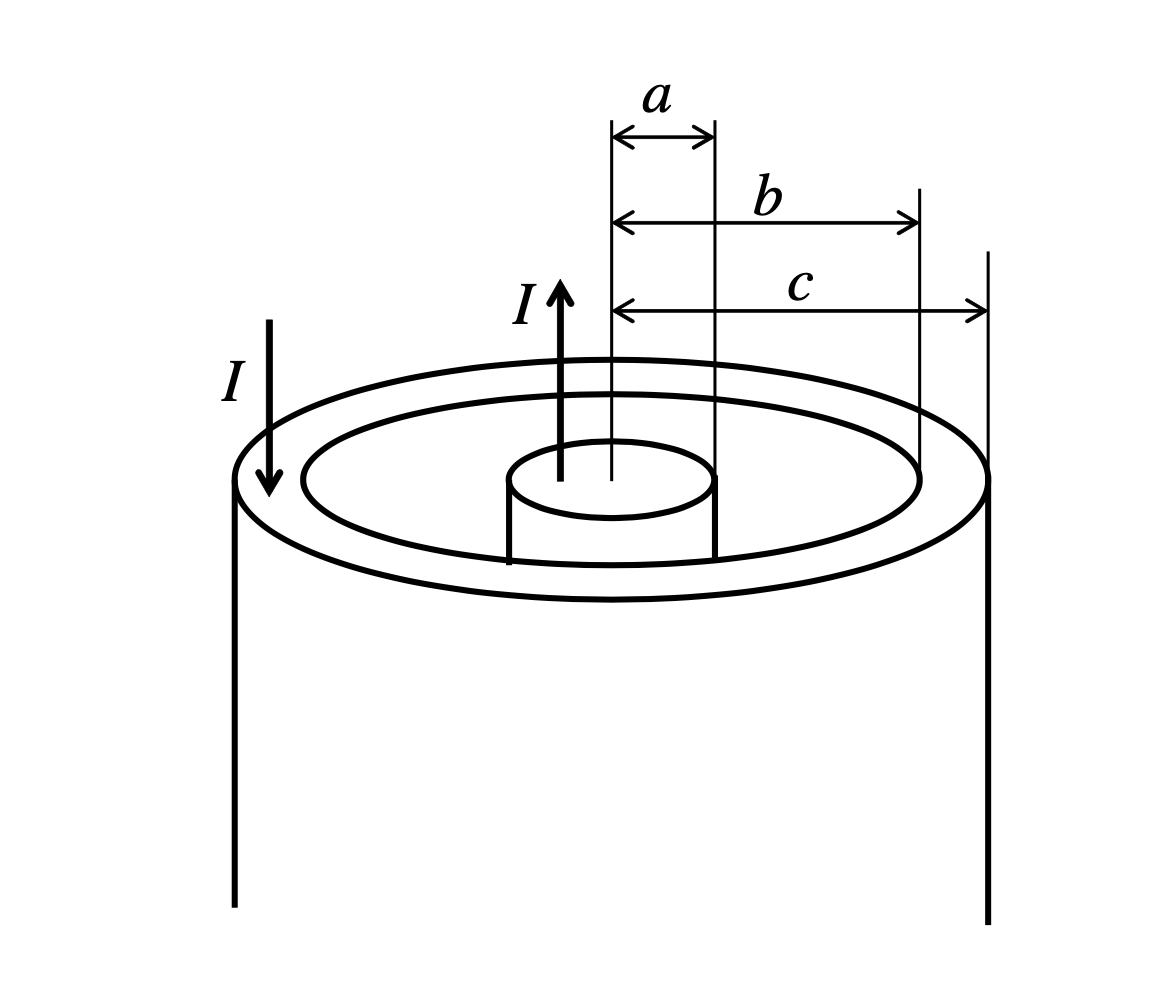
\includegraphics[scale=0.35]{./fig/R03_fig1.png}
	\caption{}
	\label{fig:1}
\end{figure}

\begin{align*}
	r>cのとき&\\
	閉曲面に流れる&電流はI-I=0であるため\\
	H&=0\,[\rm{A/m}]\\
	b<r<cのとき&\\
	dSが上向きである&ことを考慮すると\\
	\int_{C}\boldsymbol{H}\cdot d\boldsymbol{l}&=\int_{C}Hdl=2\pi rH\,[\rm{A}]\\
	\int_{S}\boldsymbol{J}\cdot d\boldsymbol{S}&=\int_{S}JdS=I-\int_{S} \frac{I}{c^{2}\pi-b^{2}\pi}dS\\
	&=I-\frac{I}{c^{2}\pi-b^{2}\pi}\pi(r^{2}-b^{2})=\left(1-\frac{r^{2}-b^{2}}{c^{2}-b^{2}}\right)I\\
	&=\left(\frac{c^{2}-b^{2}-r^{2}+b^{2}}{c^{2}-b^{2}}\right)I=\frac{c^{2}-r^{2}}{c^{2}-b^{2}}I\,[\rm{A}]\\
	2\pi r H&=\frac{c^{2}-r^{2}}{c^{2}-b^{2}}I\\
	H&=\frac{I}{2\pi r}\frac{c^{2}-r^{2}}{c^{2}-b^{2}}\,[\rm{A/m}]\\
	a<r<bのとき&\\
	同様にdSは上向き&とする\\
	\int_{C}\boldsymbol{H}\cdot d\boldsymbol{l}&=\int_{C}Hdl=2\pi rH\,[\rm{A}]\\
	\int_{S}\boldsymbol{J}\cdot d\boldsymbol{S}&=\int_{S} JdS=I\,[\rm{A}]\\
	アンペールの法則より&\\
	H&=\frac{I}{2\pi r}\,[\rm{A/m}]\\
	r<aのとき&\\
	同様にdSは上向き&とする\\
	\int_{C}\boldsymbol{H}\cdot d\boldsymbol{l}&=\int_{C}Hdl=2\pi rH\,[\rm{A}]\\
	\int_{S}\boldsymbol{J}\cdot d\boldsymbol{S}&=\int_{S} JdS=\frac{I}{a^{2}\pi}r^{2}\pi=\frac{r^{2}}{a^{2}}I\,[\rm{A}]\\
	アンペールの法則より&\\
	H&=\frac{\frac{r^{2}}{a^{2}}I}{2\pi r}=\frac{I}{2\pi a^{2}}r\,[\rm{A/m}]\\\\
	\therefore H&=
	\left\{
	\begin{matrix}
	\frac{I}{2\pi a^{2}}r\,[\rm{A/m}] &(0 < r< a)\\\\
	\frac{I}{2\pi r}\,[\rm{A/m}] & (a < r< b) \\\\
	\frac{I}{2\pi r} \frac{c^{2}-r^{2}}{c^{2}-b^{2}}\,[\rm{A/m}] & (b < r <c)\\\\
	0\,[\rm{A/m}] & (r >c)
	\end{matrix}
	\right .  \\
	ただし向きは&左回り(反時計回り)
\end{align*}

\section{\wfig{2}に示すような,単位長さ当たり$n$巻の無限長ソレノイドコイルがある.コイルに電流$I$を流したとき,コイルの周囲に発生する磁界$H$をアンペールの法則を用いて導出せよ.}

\begin{figure}[h]
	\centering
	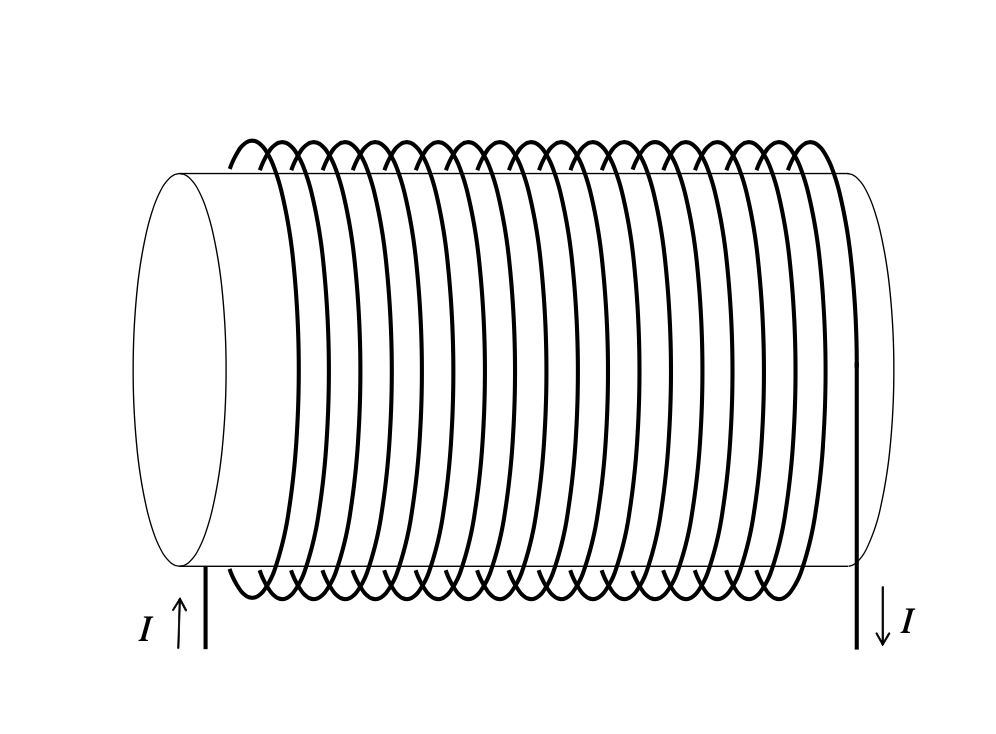
\includegraphics[scale=0.35]{./fig/R03_fig2.png}
	\caption{}
	\label{fig:2}
\end{figure}

\begin{figure}[h]
	\centering
	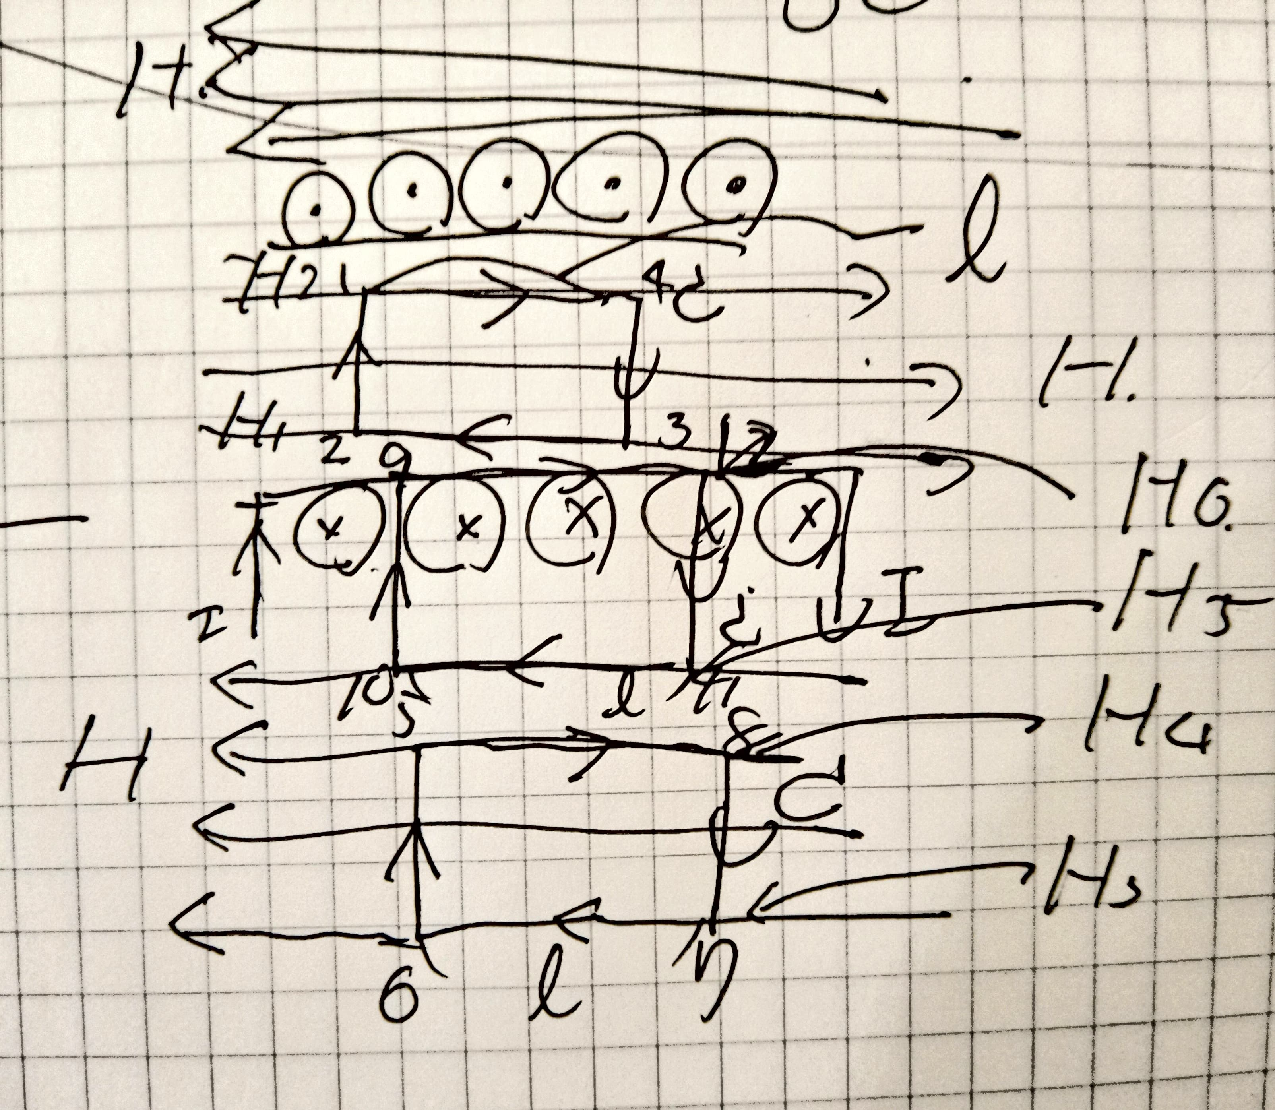
\includegraphics[scale=0.35]{./fig/fig.pdf}
	\caption{}
	\label{fig:a}
\end{figure}


\begin{align*}
このコイルによって発生する磁界はコイル&内部では右向き,コイル外部では左向きとなる.\\
経路Cとしてコイル内に&長方形1234(左上から反時計回りの順)を決める\\
また,経路23上&の磁界をH_{1},経路14上の磁界をH_{2},長さをlとする\\
\int_{C}\boldsymbol{H}\cdot d\boldsymbol{l}&=\int_{12}\boldsymbol{H}\cdot d\boldsymbol{l}+\int_{23}\boldsymbol{H}\cdot d\boldsymbol{l}+\int_{34}\boldsymbol{H}\cdot d\boldsymbol{l}+\int_{41}\boldsymbol{H}\cdot d\boldsymbol{l}\\
\boldsymbol{H}とd\boldsymbol{l}が直交するとき,&内積は0であるため\\
&=\int_{0}^{l}H_{1}dl-\int_{0}^{l}H_{2}dl\\
&=(H_{1}-H_{2})l\,[\rm{A}]\\
\int_{S}\boldsymbol{J}\cdot \boldsymbol{S}&=0\,[\rm{A}]\\
\therefore H_{1}-H_{2}&=0\\
H_{1}&=H_{2}\tag{1}\\
次に経路Cとしてコイル&外部に長方形5678(左上から反時計回りの順)を決める\\
また,経路67上&の磁界をH_{3},経路85上の磁界をH_{4},長さをlとする\\
コイル内の場合と同様の議論により&\\
\int_{C}\boldsymbol{H}\cdot d\boldsymbol{l}&=\int_{56}\boldsymbol{H}\cdot d\boldsymbol{l}+\int_{67}\boldsymbol{H}\cdot d\boldsymbol{l}+\int_{78}\boldsymbol{H}\cdot d\boldsymbol{l}+\int_{85}\boldsymbol{H}\cdot d\boldsymbol{l}\\
\boldsymbol{H}とd\boldsymbol{l}が直交するとき,&内積は0であるため\\
&=-\int_{0}^{l}H_{3}dl+\int_{0}^{l}H_{4}dl\\
&=(H_{4}-H_{3})l\,[\rm{A}]\\
\int_{S}\boldsymbol{J}\cdot \boldsymbol{S}&=0\,[\rm{A}]\\
\therefore H_{4}-H_{3}&=0\\
H_{3}&=H_{4}\\
ここでd \to \infty のときH_{4}&=0\\
\therefore H&=0\,[\rm{A/m}]\left|_{コイル外部}\right .\tag{2}\\
最後に経路Cとしてコイルの境界が経路の中心&となるような長方形9,10,11,12(左上から反時計回りの順)を決める\\
また,経路10,11上&の磁界をH_{5},経路12,9上の磁界をH_{6},長さをlとする\\
今までと同様の議論により&\\
\int_{C}\boldsymbol{H}\cdot d\boldsymbol{l}&=\int_{9,10}\boldsymbol{H}\cdot d\boldsymbol{l}+\int_{10,11}\boldsymbol{H}\cdot d\boldsymbol{l}+\int_{11,12}\boldsymbol{H}\cdot d\boldsymbol{l}+\int_{12,9}\boldsymbol{H}\cdot d\boldsymbol{l}\\
\boldsymbol{H}とd\boldsymbol{l}が直交するとき,&内積は0であり,式(2)よりコイル外部の磁界は0であるため\\
&=H_{5}l\,[\rm{A}]\\
\int_{S}\boldsymbol{J}\cdot \boldsymbol{S}&=\int_{S}JdS=nIl\,[\rm{A}]\\
\therefore H_{5}l&=nIl\\
H_{5}&=nI\,[\rm{A/m}]\\
ここでH_{5}はコイルの内部の磁界であるあるため&式(1)より\\
H&=nI\,[\rm{A/m}]\left|_{コイル内部}\right .
\end{align*}

\section{\wfig{3}に示すように,平均経路長$l$,断面積$S$,比透磁率$\mu_{r}$の鉄心に導線を$N$巻したコイルに電流$I$を流したとき,以下に示す各問いに答えよ.ただし,発生した磁界はすべて鉄心内部に存在し,漏れ磁界は存在しないものとする.}

\begin{figure}[h]
	\centering
	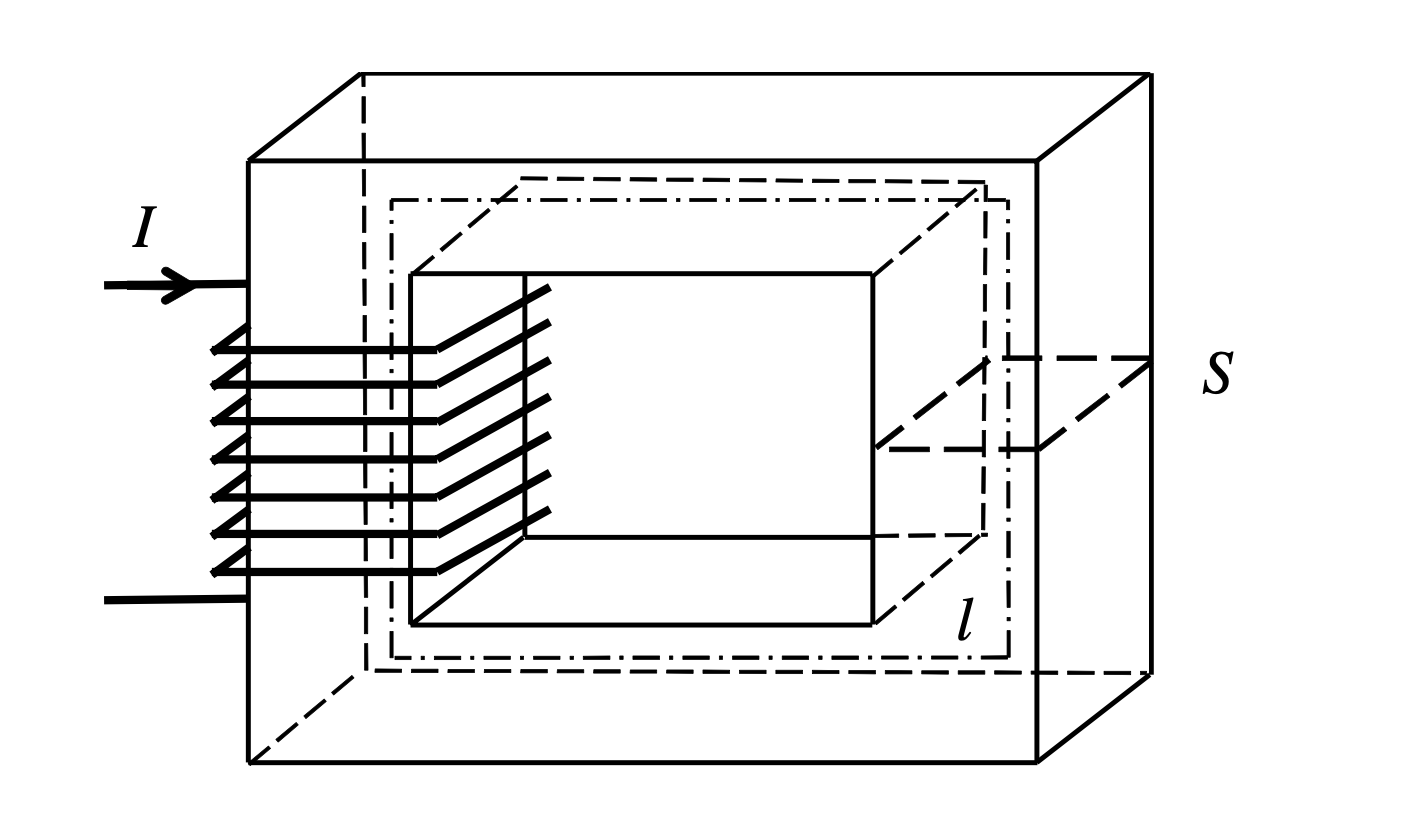
\includegraphics[scale=0.35]{./fig/co.png}
	\caption{}
	\label{fig:3}
\end{figure}

\begin{enumerate}[(a)]
	\item 発生する磁界$H$をアンペールの法則を用いて導出せよ.
	\begin{align*}
	\int_{C}\boldsymbol{H}\cdot d\boldsymbol{l}&=\int_{C}Hdl=Hl\,[\rm{A}]\\
	\int_{S}\boldsymbol{J}\cdot d\boldsymbol{S}&=\int_{S}JdS=\,[\rm{A}]\\
	\therefore H&=\,[\rm{A/m}]
	\end{align*}
	\item 鉄心内部に発生する磁束密度$B$を求めよ.
	\begin{equation*}
	B=\mu H=\mu_{0}\mu_{s}H=\,[\rm{T}]
	\end{equation*}
	\item 鉄心内部に発生する磁束$\Phi$を求めよ.
	\begin{equation*}
	\Phi=BS=\,[\rm{Wb}]
	\end{equation*}
	\item 起磁力を$NI$とすると磁気抵抗$R_{m}$は$R_{m}=\frac{NI}{\Phi}$で求められる.この鉄心の磁気抵抗$R_{m}$を求めよ.
	\begin{equation*}
	R_{m}=\frac{NI}{\Phi}=\frac{NI}{}=\frac{}{}\,[\rm{A/Wb}]
	\end{equation*}
\end{enumerate}

\section{半径$a$の無限長円柱導体に電流$I$を一様に流すと,円柱導体の周囲に発生する磁界$H$は円柱導体の中心からの距離$r$に対して図4に示すように導体内部 ($r < a$) では比例,導体外部 ($r > a$) の領域では反比例することが知られている.\\いま,円柱導体に流す電流$I$の電流密度$J$を距離$r$の関数とし,$r$の値によって電流密度を変化させると,図5に示すように導体内部($r < a$)に発生する磁界$H$を一定に保つことができる.このとき,電流密度$J$を$r$の関数として求めよ.}

\begin{figure}[h]
	\centering
	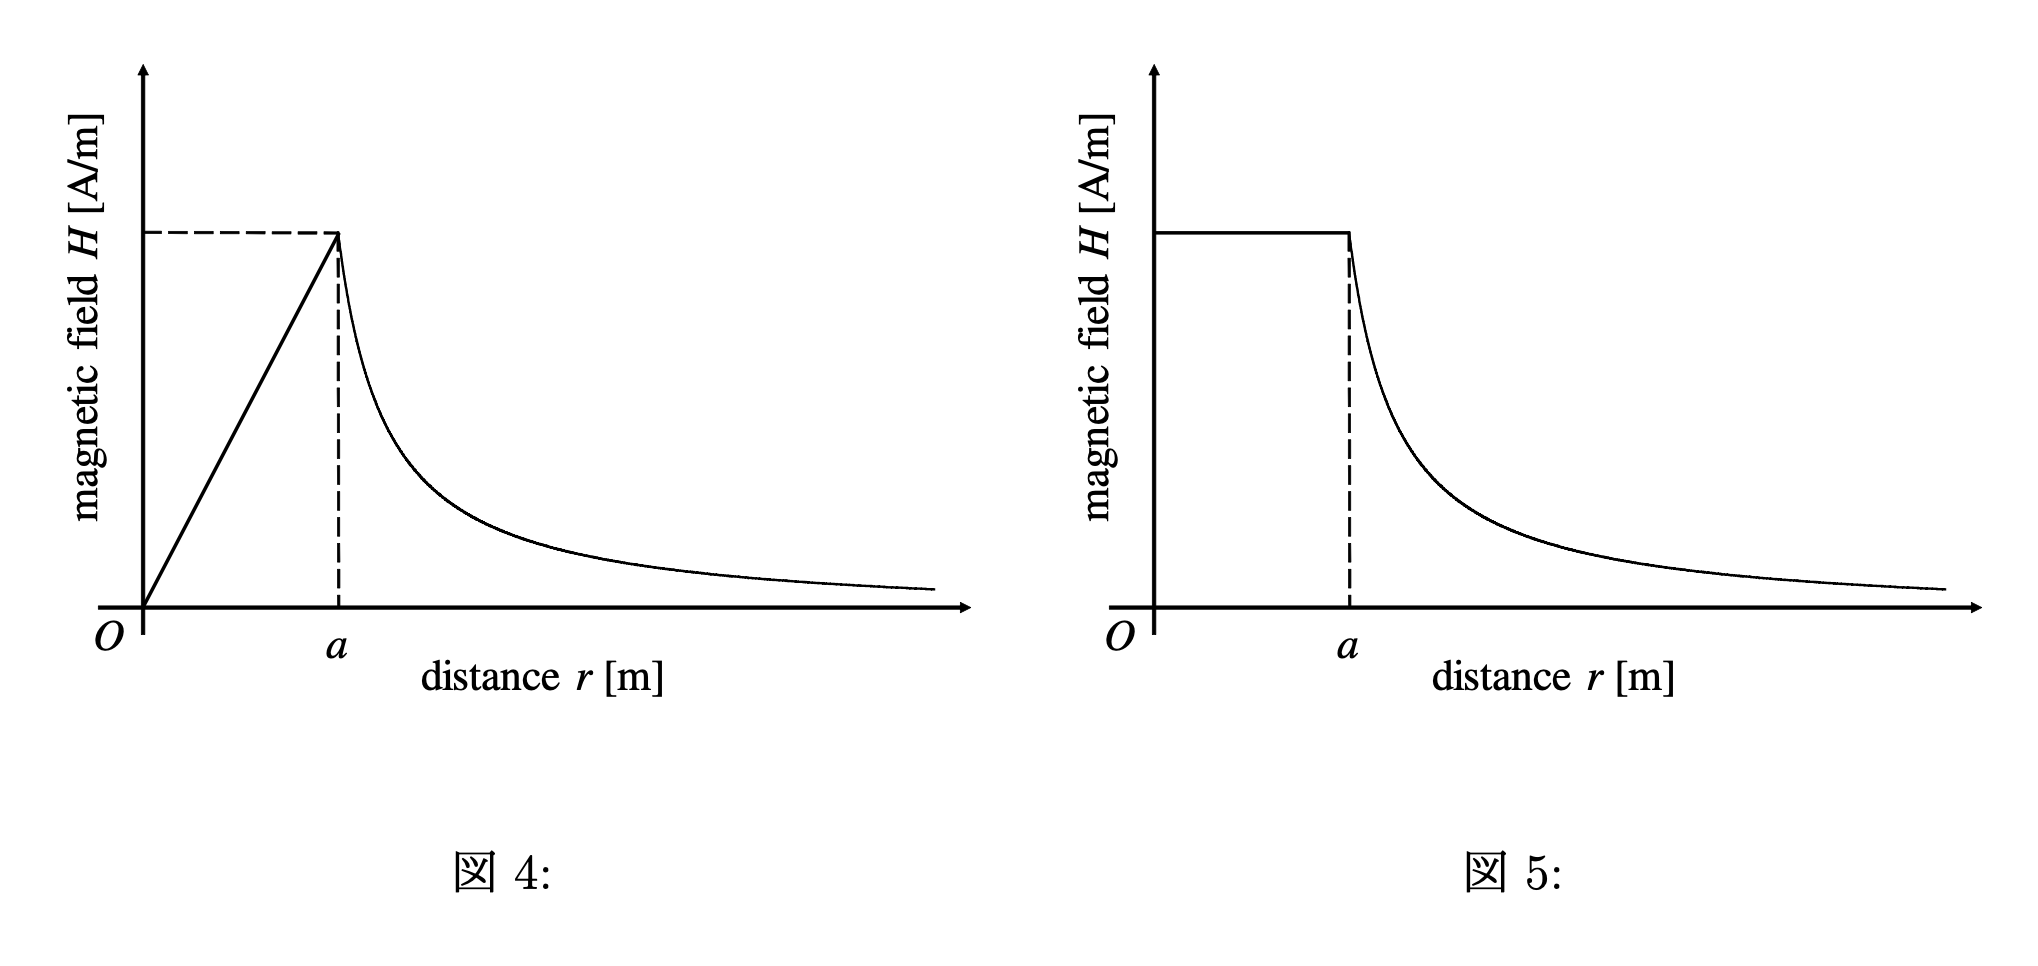
\includegraphics[scale=0.35]{./fig/e.png}
\end{figure}

\begin{align*}
\end{align*}
\end{document}